% Options for packages loaded elsewhere
\PassOptionsToPackage{unicode}{hyperref}
\PassOptionsToPackage{hyphens}{url}
%
\documentclass[
]{article}
\usepackage{amsmath,amssymb}
\usepackage{lmodern}
\usepackage{iftex}
\ifPDFTeX
  \usepackage[T1]{fontenc}
  \usepackage[utf8]{inputenc}
  \usepackage{textcomp} % provide euro and other symbols
\else % if luatex or xetex
  \usepackage{unicode-math}
  \defaultfontfeatures{Scale=MatchLowercase}
  \defaultfontfeatures[\rmfamily]{Ligatures=TeX,Scale=1}
\fi
% Use upquote if available, for straight quotes in verbatim environments
\IfFileExists{upquote.sty}{\usepackage{upquote}}{}
\IfFileExists{microtype.sty}{% use microtype if available
  \usepackage[]{microtype}
  \UseMicrotypeSet[protrusion]{basicmath} % disable protrusion for tt fonts
}{}
\makeatletter
\@ifundefined{KOMAClassName}{% if non-KOMA class
  \IfFileExists{parskip.sty}{%
    \usepackage{parskip}
  }{% else
    \setlength{\parindent}{0pt}
    \setlength{\parskip}{6pt plus 2pt minus 1pt}}
}{% if KOMA class
  \KOMAoptions{parskip=half}}
\makeatother
\usepackage{xcolor}
\usepackage[margin=1in]{geometry}
\usepackage{graphicx}
\makeatletter
\def\maxwidth{\ifdim\Gin@nat@width>\linewidth\linewidth\else\Gin@nat@width\fi}
\def\maxheight{\ifdim\Gin@nat@height>\textheight\textheight\else\Gin@nat@height\fi}
\makeatother
% Scale images if necessary, so that they will not overflow the page
% margins by default, and it is still possible to overwrite the defaults
% using explicit options in \includegraphics[width, height, ...]{}
\setkeys{Gin}{width=\maxwidth,height=\maxheight,keepaspectratio}
% Set default figure placement to htbp
\makeatletter
\def\fps@figure{htbp}
\makeatother
\setlength{\emergencystretch}{3em} % prevent overfull lines
\providecommand{\tightlist}{%
  \setlength{\itemsep}{0pt}\setlength{\parskip}{0pt}}
\setcounter{secnumdepth}{-\maxdimen} % remove section numbering
\ifLuaTeX
  \usepackage{selnolig}  % disable illegal ligatures
\fi
\usepackage[]{natbib}
\bibliographystyle{plainnat}
\IfFileExists{bookmark.sty}{\usepackage{bookmark}}{\usepackage{hyperref}}
\IfFileExists{xurl.sty}{\usepackage{xurl}}{} % add URL line breaks if available
\urlstyle{same} % disable monospaced font for URLs
\hypersetup{
  pdftitle={Test 2},
  pdfauthor={Anna Bartel},
  hidelinks,
  pdfcreator={LaTeX via pandoc}}

\title{Test 2}
\author{Anna Bartel}
\date{}

\begin{document}
\maketitle

\hypertarget{results}{%
\section{Results}\label{results}}

\hypertarget{car-fuel-economy}{%
\subsection{Car Fuel Economy}\label{car-fuel-economy}}

This dataset contains a subset of the fuel economy data that the EPA
makes available. It contains only models which has a new release every
year between 1999 and 2008 -- this was used as a proxy for the
popularity of the car.

In order to ananlyze this data, we first created a new variable that
averaged city miles per gallon and highway miles per gallon into one
composite average miles per gallon. We were interested in assessing
whether automatic or manual vehicles used more average miles per gallon.
Please review the table below:

\begin{verbatim}
## # A tibble: 2 x 3
##   transmission_type `mean avg_mpg` `sd avg_mpg`
##   <chr>                      <dbl>        <dbl>
## 1 automatic                   19.1         4.68
## 2 manual                      22.2         5.16
\end{verbatim}

We conducted a linear model where we regressed the average miles per
gallon on transmission type. Results indicate that people who drive
manual cars, on average, use more miles per gallon (M = 22.23, SD =
5.16) than people who drive automatic vehicles (M = 19.13, SD = 4.68),
t(232) = 4.60, p \textless{} .001.

\begin{verbatim}
## 
## Call:
## lm(formula = avg_mpg ~ transmission_type, data = d)
## 
## Residuals:
##      Min       1Q   Median       3Q      Max 
## -11.7273  -3.7031  -0.1789   2.8694  17.2727 
## 
## Coefficients:
##                         Estimate Std. Error t value Pr(>|t|)    
## (Intercept)              19.1306     0.3867  49.469  < 2e-16 ***
## transmission_typemanual   3.0967     0.6742   4.593 7.15e-06 ***
## ---
## Signif. codes:  0 '***' 0.001 '**' 0.01 '*' 0.05 '.' 0.1 ' ' 1
## 
## Residual standard error: 4.846 on 232 degrees of freedom
## Multiple R-squared:  0.08337,    Adjusted R-squared:  0.07941 
## F-statistic:  21.1 on 1 and 232 DF,  p-value: 7.154e-06
\end{verbatim}

Please refer to the Figure below.

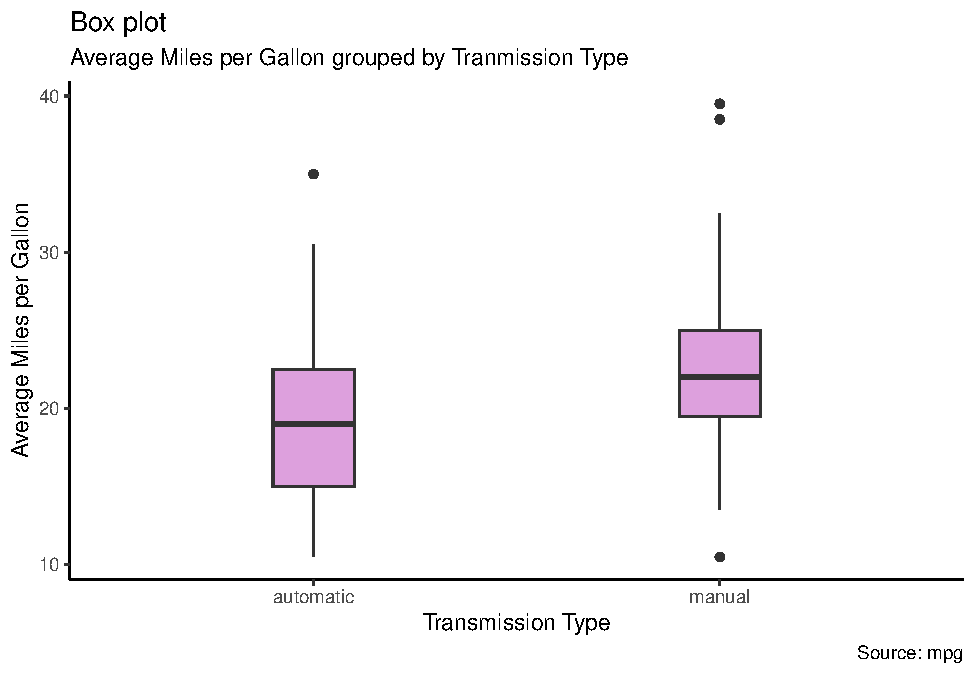
\includegraphics{TEST2_files/figure-latex/plot-1.pdf}

\end{document}
